\chapter{Der schriftliche Unterrichtsentwurf}\label{Entwurf}

Unterrichtsplanung und Unterrichtsanalyse geh\"{o}ren zum Handwerkszeug jeder Lehrkraft. Insbesondere w\"{a}hrend des Referendariats wird eine schriftliche Unterrichtsskizze verpflichtend gefordert. Im folgenden ist eine Struktur eines ausf\"{u}hrlichen Unterrichtsentwurfs nach $\to$ E. Kircher\footnote{E. Kircher, R. Girwidz, P. H\"{a}u{\ss}ler, Physikdidaktik, Springer (2015), S. 300 ff.} gegeben. Das ausf\"{u}hrliche Studium dieser Quelle sei hier dringend empfohlen. Eine verk\"{u}rzte Zusammenfassung ist im folgenden angegeben. W\"{a}hrend es im Referendariat durchaus \"{u}blich ist, eine solch ausf\"{u}hrliche Unterrichtsskizze zu erstellen und anzuwenden, beschr\"{a}nkt sich eine erfahrenere Lehrkraft auf das Erstellen einer verk\"{u}rzten \emph{Unterrichtsskizze}. Entscheidend in jeder Unterrichtsplanung ist jedoch darzustellen, wie (mit welcher Strategie, mit welchen Mitteln) man von Lernvoraussetzungen zu den Lernzielen gelangen will. Insbesondere daran wird die Qualit\"{a}t des Unterricht beurteilt! 
\mip
Nach Kircher hat ein schriftlicher Unterrichtsentwurf folgende Struktur:
\bip
\textbf{Unterrichtsentwurf} 

\begin{enumerate}
\item Vor\"{u}berlegungen

	\begin{enumerate}
	\item Lernvoraussetzungen
		\begin{enumerate}
		\item Anthropologisch-psychologische Voraussetzungen
		\item Sozio-kulturelle Voraussetzungen
		\item Spezifische Alltagsvoraussetzungen
		\end{enumerate}
	\item	Ziele ($\to$ \emph{Kapitel \ref{Ziele})}
		\begin{enumerate}
		\item Leitziele, Richtziele, Grobziele, Feinziele
		\end{enumerate}
	\item Sachanalyse ($\to$ \emph{Kapitel \ref{Elementarisierung})}
		\begin{enumerate}
		\item Fachliche Darstellung des Inhalts
		\item Elementarisierung und didaktische Rekonstruktion
		\end{enumerate}
	\item Methoden ($\to$ \emph{Kapitel \ref{Methoden})}
		\begin{enumerate}
		\item Methodische Grossformen und Unterrichtskonzepte
		\item Phasen des Unterrichts (Einstieg, Erarbeitung, Vertiefung
		\item Sozialformen
		\end{enumerate}
	\end{enumerate}

\item  Geplanter Unterrichtsverlauf (Unterrichtsskizze) 
	\\
	 Die Unterrichtsskizze ist Kernbestandteil des Unterrichtsentwurfs, der die wesentlichen Elemente einer Unterrichtsstunde oder -einheit komprimiert und \"{u}bersichtlich zusammenfasst. Ein Beispiel einer Unterrichtsskizze ist in Abbildung \ref{fig:Unterrichtsskizze} gegeben.

\item Unterrichtsmaterialien ($\to$ \emph{Kapitel \ref{Experiment},\ref{Medien})}
	\begin{enumerate}
	\item Experimente (Lehrer-/ Sch\"{u}lerexperimente
	\item Arbeitsbl\"{a}tter
	\item Tafelbild
	\end{enumerate}

\item Literatur
\end{enumerate}

\bip
Man kann deutlich erkennen, dass einem Unterrichtsentwurf ein bestimmtes $\to$ didaktisches Modell (siehe Kap. \ref{DidMod}) zugrunde gelegt wird.
\mip
Im Schulalltag beschr\"{a}nkt sich  die Unterrichtsvorbereitung im wesentlichen auf das Erstellen der Unterrichtsskizze. Hierbei handelt es sich also um eine verk\"{u}rzte und stark vereinfachte Form eines detaillierten Unterrichtsentwurfs. Sie enth\"{a}lt die wesentlichen Elemente des geplanten Unterrichts, wie zum Beispiel das Thema, die Zielsetzung, den groben Ablauf sowie die vorgesehenen Methoden und Materialien. Im Gegensatz zum ausf\"{u}hrlichen Unterrichtsentwurf wird eine Unterrichtsskizze oft in tabellarischer Form dargestellt und dient vor allem der schnellen Orientierung und Planung des Unterrichts. Sie ist n\"{u}tzlich f\"{u}r Lehrkr\"{a}fte, um den \"{U}berblick \"{u}ber die Struktur und den Verlauf der Unterrichtseinheit zu behalten, ohne dabei in die Detailtiefe eines vollst\"{a}ndigen Entwurfs zu gehen.
\bip
\textbf{Pro-Tipp:} Lehranf\"{a}nger legen die Unterrichtsskizze auf den Lehrertisch, um gelegentlich selbstbewusst einen Blick drauf zu werfen.
\bip

\begin{figure}
	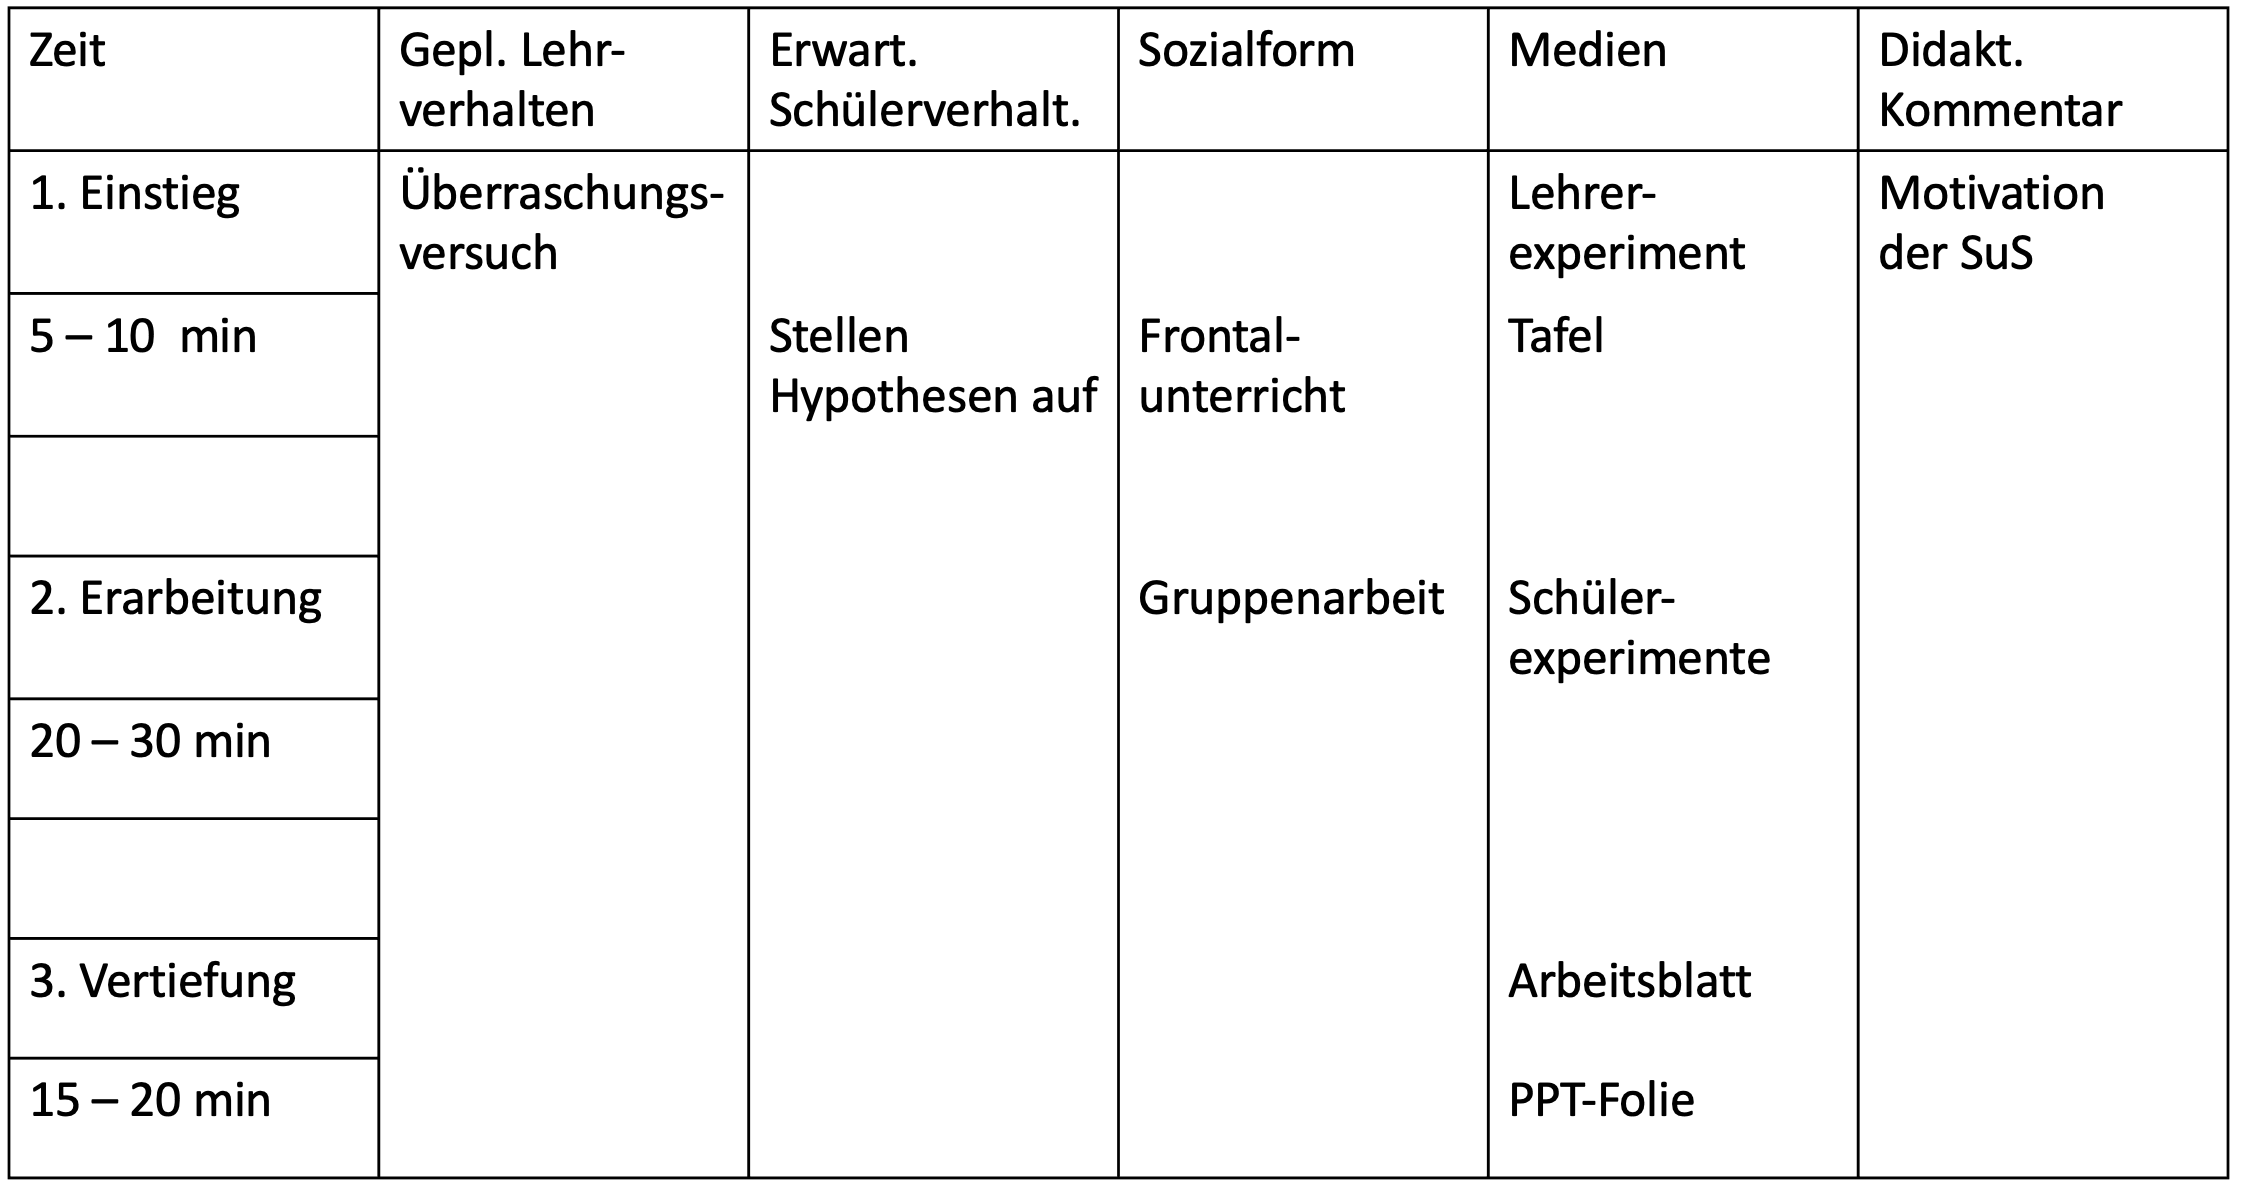
\includegraphics[scale=.2]{Unterrichtsskizze_02.png}
	\caption{Beispiel einer Unterrichtsskizze als Teil des Unterrichtsentwurfs}
	\label{fig:Unterrichtsskizze}
\end{figure}
